\chapter{Introduction}
\def\thisDir{ch01-intro}

  \section{System idenfication}

\begin{figure}

  \centering
  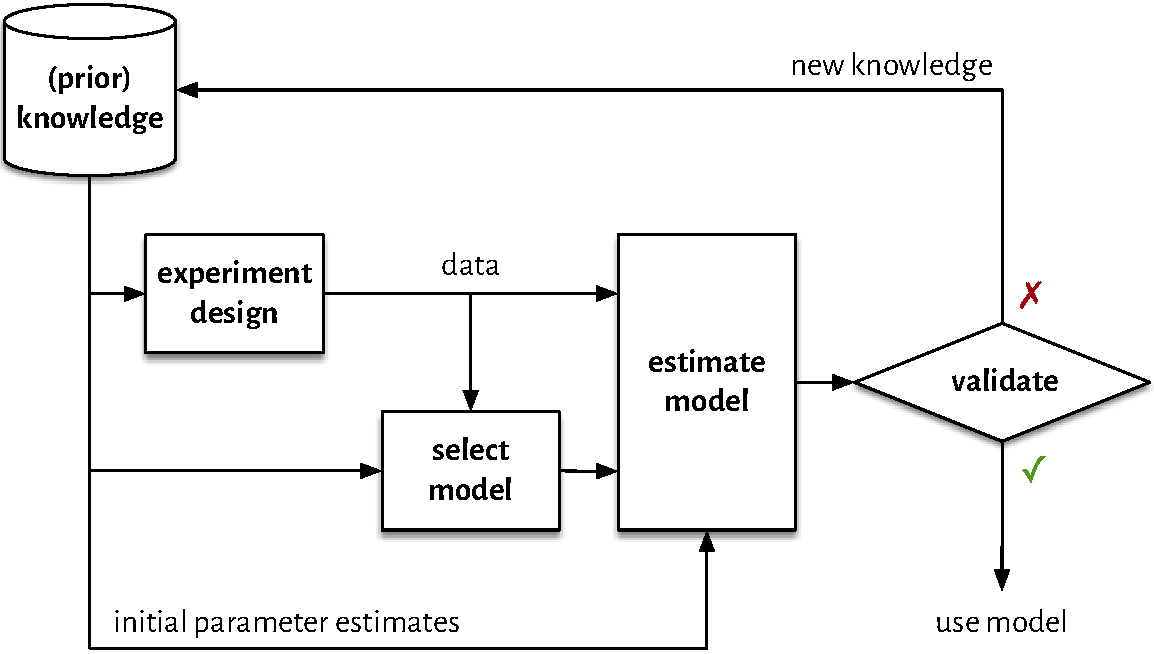
\includegraphics[width=0.9\columnwidth]{\thisDir/figs/id-cycle.pdf}
  \caption[Identification loop]{Typical system identification loop. Figure based on \citep[Figure 1.10]{Ljung1999}.}
  \label{fig:intro:identification-cycle}
\end{figure}

   \section{Contributions}

   \section{Publications}
   The lion's share of this thesis has been published either in peer-reviewed scientific journals and conferences or has been submitted to such venues at the time of writing.
   This section links my different publications to the different sections in this thesis.
   For an overview of publications grouped by type, please refer to \pageref{publicationList}.

\begin{refsection}
% http://tex.stackexchange.com/questions/38580/displaying-selected-bibliographic-items-in-the-body-of-the-text
% http://tex.stackexchange.com/questions/126226/how-do-i-instruct-fullcite-to-use-maxbibnames-rather-than-maxcitenames

\makeatletter
\DeclareCiteCommand{\fullcite}
  {\defcounter{maxnames}{\blx@maxbibnames}%
    \usebibmacro{prenote}}
  {\usedriver
     {\DeclareNameAlias{sortname}{default}}
     {\thefield{entrytype}}}
  {\multicitedelim}
  {\usebibmacro{postnote}}
\DeclareCiteCommand{\footfullcite}[\mkbibfootnote]
  {\defcounter{maxnames}{\blx@maxbibnames}%
    \usebibmacro{prenote}}
  {\usedriver
     {\DeclareNameAlias{sortname}{default}}
     {\thefield{entrytype}}}
  {\multicitedelim}
  {\usebibmacro{postnote}}
\makeatother

% http://tex.stackexchange.com/questions/18664/underline-my-name-in-the-bibliography
\DeclareNameFormat{author}{%
\ifthenelse{\equal{#1}{Geerardyn}}%
    {\textbf{\ifblank{#3}{}{#3\space}#1}}%
    {\ifblank{#3}{}{#3\space}\ifblank{#5}{}{#5\space}#1}%
\ifthenelse{\value{listcount}<\value{liststop}}%
    {\addcomma\space}
    {}}

The quasi-logarithmic multisines presented in \chapref{sec:excitation} are based on a journal article published in \gls{IEEE} Transactions on Instrumentation \& Measurement:
\begin{itemize}
  \item \fullcite{Geerardyn2013TIM}, 
\end{itemize}
preliminary results were also presented at the 2012 \gls{IFAC} symposium on System Identification (\textsc{SYSID}) and the \gls{IEEE} International Instrumentation and Measurement Conference (\textsc{I$^{\text{2}}$MTC}):
\begin{itemize}
  \item \fullcite{Geerardyn2012IMTC}, and
  \item \fullcite{Larsson2012SYSID}.
\end{itemize}
This work has also been presented at the following local (non-refereed) conferences:
\begin{itemize}
  \item \fullcite{Geerardyn2012Benelux}, and
  \item \fullcite{Geerardyn2012ERNSI}.
\end{itemize}

The non-parametric estimation methods in \chapref{sec:nonparametric} are based on a yet-unpublished journal manuscript:
\begin{itemize}
  \item \TODO{Geerardyn2016LRM}
\end{itemize}
and the truncated \gls{LPM} presented in the same chapter is based on a journal published in \gls{IEEE} Transactions on Instrumentation \& Measurement:
\begin{itemize}
  \item \fullcite{Lumori2014TIM}.
\end{itemize}
Relatedly, a preliminary study of the \gls{LPM} in the context of lightly-damped \gls{MIMO} systems has been presented at the (non-refereed) Benelux Meeting on Systems and Control:
\begin{itemize}
    \item \fullcite{Verbeke2015Benelux}.
\end{itemize}


The use of the non-parametric \gls{FRF} estimation methods for \Hinf gain estimation (and in general the \gls{FRF} interpolation from \chapref{sec:hinf}) has been presented at the 2014 \gls{IFAC} World Conference in South Africa and 
\begin{itemize}
  \item \fullcite{Geerardyn2014IFAC},
  \item \fullcite{Geerardyn2014ISMA}.
\end{itemize}
Preliminary results have been presented at local (non-refereed) conferences:
\begin{itemize}
  \item \fullcite{Geerardyn2013Benelux},
  \item \fullcite{Geerardyn2013ERNSI},
  \item \fullcite{Geerardyn2014Benelux},
  \item \fullcite{Geerardyn2014DYSCO}, and
  \item \fullcite{Geerardyn2014ERNSI}.
\end{itemize}
The experimental work related to \chapref{sec:hinf} is also presented at the 2015 \gls{IFAC} Symposium on System Identification (\textsc{SYSID}) and :
\begin{itemize}
  \item \fullcite{Voorhoeve2015}
  \item \fullcite{Voorhoeve2015ERNSI}
\end{itemize}

The study of different initialization strategies as depicted in \chapref{sec:initvals} has been published in the \gls{IEEE} Transactions on Instrumentation \& Measurement:
\begin{itemize}
  \item \fullcite{Geerardyn2015TIM},
\end{itemize}
and also at the local (non-refereed) 2015 Benelux Meeting on Systems and Control:
\begin{itemize}
    \item \fullcite{Geerardyn2015Benelux}.
\end{itemize}

In collaboration with fellow researchers, I have written a few other publications.
However, these publications are not covered in this thesis.

\begin{itemize}
  \item \fullcite{vanBerkel2014Automatica}
  \item \fullcite{Cooman2012SMACD}
  \item \fullcite{Cooman2012DYSCO}
  \item \fullcite{Cooman2012ERNSI}
\end{itemize}


\end{refsection}

